\chapter{Introduction}\label{ch1:introduction}

To get an ideal feel of 3D when we move our head what we see in terms of extent of foreground and background changes based on the change in our head pose. These changes when rendered are referred to as novel views.  

Depth maps are derived from the predicted MPIs and not predicted in parallel with the MPIs

Measure the quality of derived depth map estimated on the iBims-1 benchmark

In the abstract they say they use scale-invariant view synthesis as supervision by which they mean they use additional views of the scene  as supervision (possibly unscaled?)

Single-view view synthesis only during inference. During training 2020 model learns to predict an MPI in one stage without requiring any post-processing steps but nevertheless requires multiple images of the same scene as supervision in the one-stage training pipeline.

Single view view synthesis is an diffenert fromo the data collection aspedct of the 2018 paper becasue they retain the sparse point clouds and a record of whicvh points were tracked in each frame (refereed to as vidsible points)



% The ongoing COVID-19 pandemic has clearly contributed to a surge () not just because of the resultant stay-at-home/work-form-home and the resulting work from home scenarios orders but also because of the increase in the rate of concern of people about their acquaintances and loved ones alike. From the most important work meeting to the casual conversations with friends/family people are using applications like FaceTime, Zoom, 

At this point in humanity's technological progress, one can likely see novel view (image taken from a certain viewpoint) synthesis --- generating new views of a scene using a given set of one or more images of the same scene --- to be a constantly evolving solution to a variety of problems <<<<<like what???>>>>> far into the future.

<<<< Display devices like VR headsets are functionally holographic --- as the user moves around they have to have new perspectives for each position that they are in; and in order to serve that you have to have something fundamentally holographic. Moreover we're also getting this on 2D screens: multiperspective panels. So it's not that far off before all your phones and computers and TVs are going to be multiperspective too, at which point 2D images are going to look kind of uninteresting by comparison. Like comparing today's newspapers with the fictional Wizarding World's newspaper, The Daily Prophet. https://youtu.be/BXdKVisWAco >>>>>



Currently, (novel) view synthesis cannot be achieved end-to-end without going from the given image(s) to some form of an intermediate representation of the the structure of the scene depicted by the given image(s), and onto the final synthesized/rendered image.

given image ---> intermediate representation ---> final synthesized image

One of the latest variations of such an intermediate representation is called a Multiplane Image (MPI) --- first introduced by <<<<<<Richard Tucker, et. al.>>> in the <<<<2018 SIGGRAPH paper>>>>.

\section{Multiplane Images}

MPI scene representation is similar to Layered Depth Image (LDI) scene representation introduced by <<<Shade et at 1998>>>

They both consist of a series of fronto-parallel planes \ref{mpi-layered-representation} that are at different depths from the reference camera of one of the given images. These planes contain the RGB information of the original pixels of the image(s) segregated according to depth.

<<<<<<TODO>>>>> The difference between LDI and MPI -MPI HAS ALPHA - masking effects can be generated with alpha transparency
<<<<<TODO>>>>> how do LDI/MPI represent layered depth

how do they even come up with depth pixels for both LDI/MPI? do they already know depth from ground truth ????
and how do they calculate depth ???

we can give the number of layers to the network - does it make a difference? 
when you have more layers you get more depth info - more clarity in the rendered image - <<<<<RESULTS/DISCUSSIONS>>>>

<<<<<TODO>>>>
eseentially simplify the mpi papers for the readers
be clear about whay a certain choice was made - like number of layers 
system - algorithms - choices - reasons for these choices 
just like hyperparameter tuning 
<<<<<TODO>>>>>>

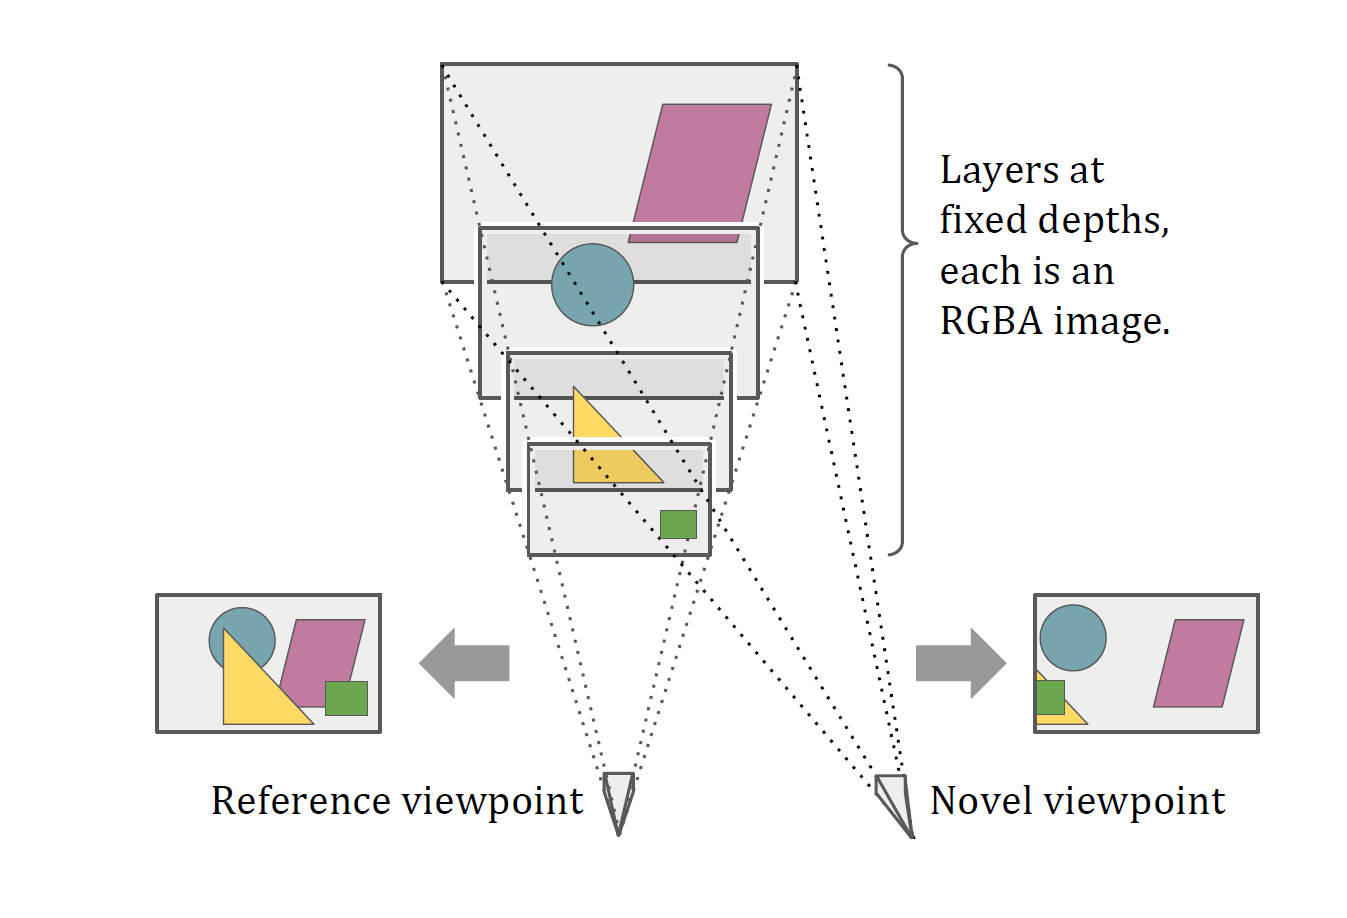
\includegraphics{figures/mpi-layered-representation.png}\label{fig:mpi-layered-representation}

3 paragraphs or clarity

\section{Generating Novel Views using MPI}

Similar to how supervised machine learning can be used to learn how to infer novel views by capturing images of a large number of scenes, withholding some
<<<<<<<views of each scene as ground truth, training a model that predicts
such missing views from one or more given views, and comparing
these predicted views to the ground truth as the loss or objective
that the learning seeks to optimize. Recent>>>>>>>>

\section{Hypotheses}

 hypotheses of this thesis are as follows:
1) Te MPI 2020 paper, which produces good disparity maps for <the opposite of close-up shots> <long shots of objects/landscapes> \cite{}, is unable to do so for close-up shot of people/objects. When we re-recreated the 202 Hence, our first hypothesis is that re-retraining the re-created 2020 MPI model on  

\section{Contributions/Overview}


\input{chapters/ch1-introduction/background}
https://mashable.com/video/google-project-starline-3d-video-calls

somehow quantizing the depths 
tyhe 3d objecxt wiil fall in different plab=nes

why did they include colmap point could vs 

 Sec A: 

From the most important work meetings to the casual conversations with friends/family, people are using applications like FaceTime, Zoom and Google Meet. One way of improving video chat experience is to bring in the feel of 3D by providing alternate views of the viewed scene rendered at different viewpoints. To fortify the 3D experience the rendered novel view needs to match the head pose of the viewer. 


Fig. 1: Figure to describe how novel views can improve video chat experience. 

Currently, novel view synthesis cannot be achieved end-to-end without some form of an intermediate representation of the structure of the scene depicted by the given image(s). One of the latest variations of such an intermediate representation is called a Multiplane Image (MPI) --- first introduced by <<<<<<Richard Tucker, et. al.>>> in the <<<<2018 SIGGRAPH paper>>>>.

Fig. 2: given image ---> intermediate representation ---> final synthesized image



------------------------------------

\section{Multiplane Images}

MPI scene representation is similar to Layered Depth Image (LDI) scene representation introduced by <<<Shade et at 1998>>>.

Both [][] consist of a series of fronto-parallel planes \ref{mpi-layered-representation} that are at different depths from the reference camera of one of the given images. These planes contain the RGB information of the original pixels of the image(s) segregated according to depth. The difference between LDI and MPI is that MPI HAS ALPHA masking effects can be generated with alpha transparency and MPI has fixed depth. 



------------------------------------




\chapter{Introduction}\label{ch1:introduction}

% The ongoing COVID-19 pandemic has clearly contributed to a surge () not just because of the resultant stay-at-home/work-form-home and the resulting work from home scenarios orders but also because of the increase in the rate of concern of people about their acquaintances and loved ones alike. From the most important work meeting to the casual conversations with friends/family people are using applications like FaceTime, Zoom, 

At this point in humanity's technological progress, one can likely see novel view (image taken from a certain viewpoint) synthesis --- generating new views of a scene using a given set of one or more images of the same scene --- to be a constantly evolving solution to a variety of problems <<<<<like what???>>>>> far into the future.

<<<< Display devices like VR headsets are functionally holographic --- as the user moves around they have to have new perspectives for each position that they are in; and in order to serve that you have to have something fundamentally holographic. Moreover we're also getting this on 2D screens: multiperspective panels. So it's not that far off before all your phones and computers and TVs are going to be multiperspective too, at which point 2D images are going to look kind of uninteresting by comparison. Like comparing today's newspapers with the fictional Wizarding World's newspaper, The Daily Prophet. https://youtu.be/BXdKVisWAco >>>>>

Currently, (novel) view synthesis cannot be achieved end-to-end without going from the given image(s) to some form of an intermediate representation of the the structure of the scene depicted by the given image(s), and onto the final synthesized/rendered image.

given image ---> intermediate representation ---> final synthesized image

One of the latest variations of such an intermediate representation is called a Multiplane Image (MPI) --- first introduced by <<<<<<Richard Tucker, et. al.>>> in the <<<<2018 SIGGRAPH paper>>>>.

\section{Multiplane Images}

MPI scene representation is similar to Layered Depth Image (LDI) scene representation introduced by <<<Shade et at 1998>>>

They both consist of a series of fronto-parallel planes \ref{mpi-layered-representation} that are at different depths from the reference camera of one of the given images. These planes contain the RGB information of the original pixels of the image(s) segregated according to depth.

<<<<<<TODO>>>>> The difference between LDI and MPI -MPI HAS ALPHA - masking effects can be generated with alpha transparency
<<<<<TODO>>>>> how do LDI/MPI represent layered depth

how do they even come up with depth pixels for both LDI/MPI? do they already know depth from ground truth ????
and how do they calculate depth ???

we can give the number of layers to the network - does it make a difference? 
when you have more layers you get more depth info - more clarity in the rendered image - <<<<<RESULTS/DISCUSSIONS>>>>

<<<<<TODO>>>>
eseentially simplify the mpi papers for the readers
be clear about whay a certain choice was made - like number of layers 
system - algorithms - choices - reasons for these choices 
just like hyperparameter tuning 
<<<<<TODO>>>>>>

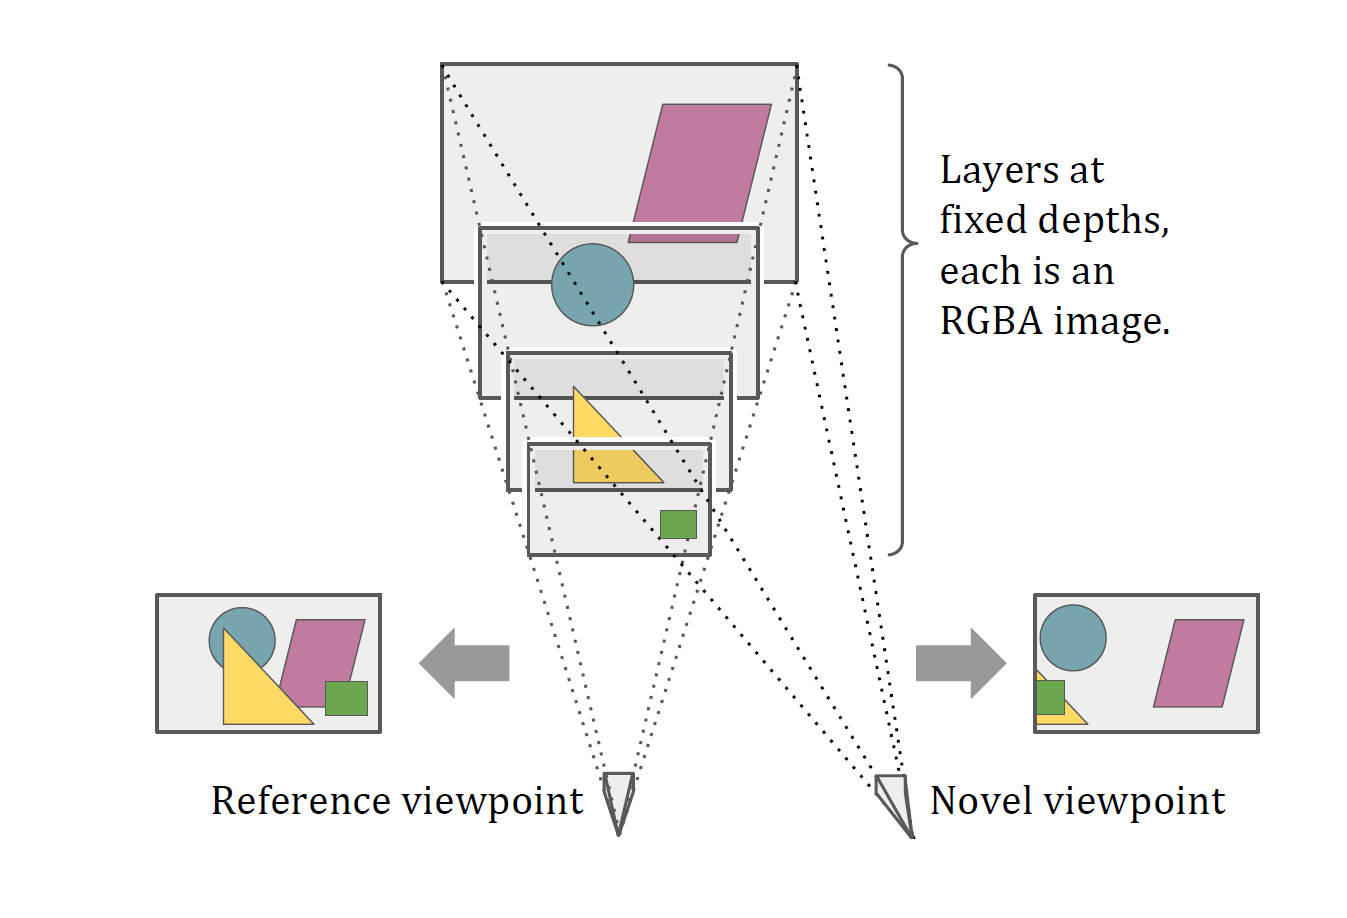
\includegraphics{figures/mpi-layered-representation.png}\label{fig:mpi-layered-representation}

3 paragraphs or clarity

\section{Generating Novel Views using MPI}

Similar to how supervised machine learning can be used to learn how to infer novel views by capturing images of a large number of scenes, withholding some
<<<<<<<views of each scene as ground truth, training a model that predicts
such missing views from one or more given views, and comparing
these predicted views to the ground truth as the loss or objective
that the learning seeks to optimize. Recent>>>>>>>>

\section{Hypotheses}

 hypotheses of this thesis are as follows:
1) Te MPI 2020 paper, which produces good disparity maps for <the opposite of close-up shots> <long shots of objects/landscapes> \cite{}, is unable to do so for close-up shot of people/objects. When we re-recreated the 202 Hence, our first hypothesis is that re-retraining the re-created 2020 MPI model on  

\section{Contributions/Overview}


\input{chapters/ch1-introduction/background}
https://mashable.com/video/google-project-starline-3d-video-calls

somehow quantizing the depths 
tyhe 3d objecxt wiil fall in different plab=nes

why did they include colmap point could vs 




___________________________________________________________________________




\section{Background}\label{sec1:background}

Multiplane images were first repurposed in the 2018 Stereo Magniification: Learning View Synthesis using Multiplane Images paper \cite{}

The MPI generation convolutional neural network 

<<<<<pose refers to position + orientation throughout this paper>>>>>

In the 2018 original MPI paper, a stereo pair of images is used to predict the MPI in the following manner:

\begin{itemize}
    \item The viewpoint of one of the stereo pair (I1, I2) I1 is used as the reference viewpoint for the MPI to be predicted
    \item Hence the MPI would be fronto-parallel to the reference coordinate plane of I1, with all its planes stacked parallel to one another facing the camera of I1.
    \item The input to the network is I1, its camera parameters c1
\end{itemize}

\chapter{Related Work}\label{ch2:related-work}
related work augmenting video chat 

augmenting view synthesis


augmenting head pose estimation

get closer to using view synthesis in video chat 

https://ieeexplore.ieee.org/document/9105988
This paper has a similar theme as the current thesis but differs mainly, in that, it has it renders 3D video using an intermediate light field representation as opposed to the current Multiplane Representation

https://www.sciencedirect.com/science/article/pii/S2090447919301297




Stereo Magnification (2018) paper introduces the MPI representation and also explains how the data was processed. Some parts of the code are refactored and reused in the 2020 MPI paper like how the 2018 paper loads data in: in particular the data loader (loader.py, datasets.py) does subsequence selection and some slight random cropping. There are several more interesting MPI-related papers (Pushing the Boundaries, DeepView, Local Lightfield Fusion) which explore different directions, but none of them are tackling the single-view approach.

From the code the 2020 MPI authors have released (https://github.com/google-research/google-research/tree/master/single_view_mpi) we can see:
  • their network definition (convolutional layers, kernel sizes, etc) (nets.mpi_from_image)
  • how to render views from new camera positions (mpi.render), including everything related to the homography, etc

What we didn't have was (a) the implementation of the losses, and (b) data including point clouds and a way to load it in.
One of the key points of Single-View View Synthesis was to use sparse point cloud data to make the view synthesis loss scale-invariant. To obtain such data we would have to process the mannequin dataset to obtain point cloud and/or depth, for example with COLMAP, and then we could write a data loader or extend the one from Stereo Magnification.

The original Mannequin Dataset (https://google.github.io/mannequinchallenge/www/index.html) is quite a bit smaller than RealEstate10K, and so there is a risk of overfitting. Hence, we are trying to find if it is better to use a combination of both RealEstate and MannequinChallenge than just MannequinChallenge alone). Hence this was one next step after we were able to figure out how to train the 2020 MPI paper model.









